\documentclass[oldfontcommands,twoside,a4paper,12pt]{article} 
\usepackage{xunicode}%packages de base pour utiliser xetex
\usepackage{fontspec}
\usepackage{natbib}
\usepackage{booktabs}
\usepackage{xltxtra} 
\usepackage{longtable}
\usepackage{tangutex2} 
%\usepackage{tangutex4} 
\usepackage{polyglossia} 
\usepackage[table]{xcolor}
\usepackage{color}
\usepackage{multirow}
\usepackage{gb4e} 
\usepackage{multicol}
\usepackage{graphicx}
\usepackage{float}
\usepackage{hyperref} 
\hypersetup{bookmarks=false,bookmarksnumbered,bookmarksopenlevel=5,bookmarksdepth=5,xetex,colorlinks=true,linkcolor=blue,citecolor=blue}
\usepackage{memhfixc}
\usepackage{lscape}
\usepackage[footnotesize,bf]{caption}


%%%%%%%%%%%%%%%%%%%%%%%%%%%%%%%
\setmainfont[Mapping=tex-text,Numbers=OldStyle,Ligatures=Common]{Charis SIL} 
\setsansfont[Mapping=tex-text,Ligatures=Common,Mapping=tex-text,Ligatures=Common,Scale=MatchLowercase]{Lucida Sans Unicode} 
 


\newfontfamily\phon[Mapping=tex-text,Ligatures=Common,Scale=MatchLowercase,FakeSlant=0.3]{Charis SIL} 
\newfontfamily\phondroit[Mapping=tex-text,Ligatures=Common,Scale=MatchLowercase]{Doulos SIL} 
\newfontfamily\greek[Mapping=tex-text,Ligatures=Common,Scale=MatchLowercase]{Doulos SIL} 
\newcommand{\ipa}[1]{{\phon\textbf{#1}}} 
\newcommand{\ipab}[1]{{\phon #1}}
\newcommand{\ipapl}[1]{{\phondroit #1}} 
\newcommand{\captionft}[1]{{\captionfont #1}} 
\newfontfamily\cn[Mapping=tex-text,Ligatures=Common,Scale=MatchUppercase]{MingLiU}%pour le chinois
\newcommand{\zh}[1]{{\cn #1}}
\newcommand{\tgf}[1]{\mo{#1}}
\newfontfamily\mleccha[Mapping=tex-text,Ligatures=Common,Scale=MatchLowercase]{Galatia SIL}%pour le grec
\newcommand{\grec}[1]{{\mleccha #1}}

\newcommand{\acc}{\textsc{acc}}
\newcommand{\antierg}{\textsc{antierg}}
\newcommand{\allat}{\textsc{all}}
\newcommand{\aor}{\textsc{aor}}
\newcommand{\assert}{\textsc{assert}}
\newcommand{\auto}{\textsc{auto}}
\newcommand{\caus}{\textsc{caus}}
\newcommand{\classif}{\textsc{class}}
\newcommand{\concessif}{\textsc{concsf}}
\newcommand{\comit}{\textsc{comit}}
\newcommand{\conj}{\textsc{conj}}
\newcommand{\const}{\textsc{const}}
\newcommand{\conv}{\textsc{conv}}
\newcommand{\cop}{\textsc{cop}}
\newcommand{\dat}{\textsc{dat}}
\newcommand{\dem}{\textsc{dem}}
\newcommand{\detm}{\textsc{det}}
\newcommand{\dir}{\textsc{dir1}}
\newcommand{\du}{\textsc{du}}
\newcommand{\duposs}{\textsc{du.poss}}
\newcommand{\dur}{\textsc{dur}}
\newcommand{\erg}{\textsc{erg}}
\newcommand{\evd}{\textsc{evd}}
\newcommand{\fut}{\textsc{fut}}
\newcommand{\gen}{\textsc{gen}}
\newcommand{\hypot}{\textsc{hyp}}
\newcommand{\ideo}{\textsc{ideo}}
\newcommand{\imp}{\textsc{imp}}
\newcommand{\impf}{\textsc{ipfv}}
\newcommand{\instr}{\textsc{instr}}
\newcommand{\intens}{\textsc{intens}}
\newcommand{\intrg}{\textsc{intrg}}
\newcommand{\inv}{\textsc{inv}}
\newcommand{\irreel}{\textsc{irr}}
\newcommand{\loc}{\textsc{loc}}
\newcommand{\med}{\textsc{med}}
\newcommand{\negat}{\textsc{neg}}
\newcommand{\neu}{\textsc{neu}}
\newcommand{\nmlz}{\textsc{nmlz}}
\newcommand{\nonps}{\textsc{n.pst}}
\newcommand{\opt}{\textsc{dir2}}
\newcommand{\perf}{\textsc{pfv}}
\newcommand{\pl}{\textsc{pl}}
\newcommand{\plposs}{\textsc{pl.poss}}
\newcommand{\poss}{\textsc{poss}}
\newcommand{\pot}{\textsc{pot}}
\newcommand{\prohib}{\textsc{prohib}}
\newcommand{\pst}{\textsc{pst}}
\newcommand{\recip}{\textsc{recip}}
\newcommand{\redp}{\textsc{redp}}
\newcommand{\refl}{\textsc{refl}}
\newcommand{\sg}{\textsc{sg}}
\newcommand{\sgposs}{\textsc{sg.poss}}
\newcommand{\stat}{\textsc{stat}}
\newcommand{\topic}{\textsc{top}}
\newcommand{\volit}{\textsc{vol}}

\newcommand{\racine}[1]{\begin{math}\sqrt{#1}\end{math}} 
\newcommand{\grise}[1]{\cellcolor{lightgray}\textbf{#1}} 

\begin{document}
  \title{Harmonization and disharmonization of affix ordering and basic word order\footnote{I wish to express gratitude to my language consultants: Chen Zhen and Dpal-can for Japhug (2002-present), Dpal-ldan for Situ (2012) and Ngag-dbang for Pumi (2009). I also thank Anton Antonov, Scott DeLancey, Antoine Guillaume, Alexis Michaud, Waltraud Paul, Laurent Sagart, Lameen Souag, Wu Tong, John Whitman as well as three anonymous reviewers for useful comments and corrections. This research was funded by the ANR-Corpus HimalCo, the Labex EFL (Empirical Foundations of Linguistics, GD1, Typology and annotation of information structure and grammatical relations and the International joint field survey of the rGyalrongic languages, supported by MEXT/JSPS Overseas Fieldwork Grant (2009-2012). The glosses follow the Leipzig Glossing Rules, except for the following: \textsc{autoben} autobenefactive-spontaneous, \textsc{cisloc} cislocative,  \textsc{const} constative, \textsc{hort} hortative, \textsc{inv} inverse,  \textsc{transloc} translocative}}
 
\author{Guillaume Jacques}
\maketitle


\textbf{Abstract}: Cross-category harmony (correlations between basic word order and preference for suffixes or prefixes) has been proposed by several typologists and psycholinguists as a principle to explain some apparent cross-linguistic tendencies. This paper attempts to test  whether cross-category harmony has an observable  influence on morphosyntactic change, and reviews cases of harmonization and disharmonization of affix order. The grammaticalization of associated motion prefixes in Japhug Rgyalrong, a verb-final language, constitutes a solid case of development of a disharmonious construction out of a harmonious one, and runs counter to the idea that head ordering principles have a direct effect on language change.

\textbf{Keywords}: word order typology, Associated motion, Japhug, Rgyalrong, prefixes, verbal template, Athabaskan, Ket


 

  \section{Introduction}
Nearly fifty years ago, \citet[93]{greenberg66} noticed several correlations between basic word order (OV vs. VO), the position of adpositions relative to nouns (prepositions vs. postpositions), and the preference for  suffixes vs. prefixes.  In his original formulation:
 
\begin{exe}
\ex \label{ex:greenberg}
\glt 3. Languages with dominant VSO order are always prepositional.
\glt 4. With overwhelmingly greater than chance frequency, languages with normal SOV order are postpositional.
\glt 27. If a language is exclusively suffixing, it is postpositional; if it is exclusively prefixing, it is
prepositional.
\end{exe}

Greenberg did not  mention a direct correlation between basic order at clause level and affix order, but this step was taken by some of his followers such as  \citet{vennemann74analogy} and \citet{lehmann73structural}, both of whom based their observations on data from Indo-European. To quote  \citet[23]{lehmann78typology}: ``[...]  it has been clear for some time that VSO languages are characterized by prefixation and OV languages by suffixation''.


Lehmann's observation is confirmed by the larger sample of data available from the WALS database. By combining the data in chapters 26 (\citealt{dryer11chapter26}) and 83 (\citealt{dryer11ov}) on prefixing vs. suffixing inflectional morphology and OV vs. VO order respectively, we obtain the following figures:\footnote{Not all authors would agree with the WALS values in particular concerning SOV vs. SVO for  many individual languages (see for instance \citealt{plank09wals} concerning German). }

\begin{table}[H]

\caption{Correlation between OV order and prefixing vs. suffixing inflectional morphology (data from WALS); each row in the table adds up to 100\%} \label{tab:wals}
\resizebox{\columnwidth}{!}{
\begin{tabular}{llllllllll}
\toprule
 &	  	OV   &&	VO  &&	No &dominant order &Total \\
 \midrule
Little affixation  & 	35 & 	(25.0\%) & 	100 & 	(71.4\%) & 	5 & 	(3.6\%) & 	140 & 	(14.8\%) \\ 
Strongly suffixing  & 	269 & 	(68.6\%) & 	93 & 	(23.7\%) & 	30 & 	(7.7\%) & 	392 & 	(41.5\%) \\ 
Weakly suffixing  & 	70 & 	(57.9\%) & 	44 & 	(36.4\%) & 	7 & 	(5.8\%) & 	121 & 	(12.8\%) \\ 
Equal prefixing and suffixing  & 	49 & 	(34.5\%) & 	78 & 	(54.9\%) & 	15 & 	(10.6\%) & 	142 & 	(15\%) \\ 
Weakly prefixing  & 	23 & 	(25.0\%) & 	61 & 	(66.3\%) & 	8 & 	(8.7\%) & 	92 & 	(9.7\%) \\ 
Strongly prefixing  & 	6 & 	(10.3\%) & 	52 & 	(89.7\%) & 	 & 	(0.0\%) & 	58 & 	(6.1\%) \\ 
\midrule
 & 	452 & 	(47.8\%) & 	428 & 	(45.3\%) & 	65 & 	(6.9\%) & 	945 & 	(100\%) \\ 
\bottomrule
\end{tabular}}
\end{table}
We observe from this table that there are more weakly and strongly suffixing OV languages than VO languages (339 vs. 137) and fewer weakly and strongly prefixing OV languages than VO languages (29 vs. 113). 


 

This table also illustrates the well-known fact that suffixes are more widespread than prefixes (\citealt[67]{sapir21language}): even with VO order, mainly prefixing languages are   slightly less common than mainly suffixing ones (113 vs. 137).

 \citet{vennemann74analogy}   first attempted to explain these tendencies in terms of the \textit{Natural Serialization Principle}, in other words the idea that languages tend to develop toward more consistent order between Head and Dependent. A similar idea was put forth by \citet[227]{hawkins88prefixing}, who also added a second principle to account for the suffixing preference:
\begin{exe}
\ex \label{ex:hawkins}
\begin{xlist}[(ii)]
\exi{(a)} 
\glt \textbf{The Head Ordering Principle}: The affixal head of a word is ordered on the same side of its
subcategorized modifier(s) as P is ordered relative to NP within PP, and as V is ordered relative to a direct object NP.
\exi{(b)} 
\glt \textbf{Processing preference for suffixing}:
Lexical recognition precedes syntactic processing, so language users will prefer to process stems before affixes. Stem-affix order provides the most efficient structure for processing.
   \end{xlist}
\end{exe}



While these psycholinguistic models have their merits, they do not constitute the only possible logical explanations for the observed correlation between OV order and affix position. Three other possibilities should be taken into account.

First, these observed patterns might be the result of diachronic processes rather than of a synchronic cognitive constraint (\citealt{bybee88dia}, \citealt{mithun03prefixes}). As pointed out by \citet[178]{mithun03prefixes}: ``It is not unlikely that observed cross-category harmony is more often an artifact of regular processes of language change than the product of a synchronic force.'' This idea has been supported by several scholars, in particular  \citet[2]{creissels08alignment}: ``contrary to what functional approaches to language typology often suggest, it does not always make sense to postulate direct functional explanations for the types of organization attested in the languages of the world, since at least some types of organization may develop in a purely mechanical fashion as a by-product of developments in other areas of grammar.''

 In this perspective, the rarity of certain patterns is due either (a) to the near-absence of possible grammaticalization pathways leading to the creation of a given structure, or (b) to the instability of a given structure, which could only be maintained for a short period of time.

 Notice however that both (a) and (b) do not necessarily contradict the cognitive hypothesis: one can argue that the cognitive constraints also apply to diachronic processes. For instance, \citet[166]{hall92morpho} proposes that ``The hypothesised universal psycholinguistic dispreference for prefixing must, it seems, be instantiated in particular languages word by word by a mechanism which, given the right conditions, `blocks' the fusion of potential prefixes with free stems." In other words, under this hypothesis the cognitive constraints in (\ref{ex:hawkins}) could either hinder the grammaticalization of a given structure, or contribute to its rapid demise. Mithun's or Creissels' arguments are therefore valid only if one can prove that a given diachronic change is purely mechanical and functionally unmotivated.
 
 
 Second, it has been argued that factors such as prosodic typology (trochaic vs. iambic structure) might affect the preference for prefixes or suffixes (see \citealt{donegan04munda} and a historical overview of this issue by \citealt{plank98covariation}). \citet{lahiri10phrasing} have also proposed that in Germanic, where function words consistently precede lexical words, a preference for encliticization can be observed.
 No generalization on the typology of historical morphological developments can neglect the prosodic factor.


Third, these tendencies might be the product of historical contingency, the unusual patterns being rare not because of a cognitive disadvantage, but because some typological features spread through language replacement and language contact, and erased a former greater diversity, especially in Eurasia.  This hypothesis is supported by recent research such as \citet{dunn11word.order}, who propose that dependencies between typological features are mainly areal or family-specific.

 
 The historical contingency hypothesis makes no particular prediction: if true, it implies that most if not all observed correlations between typological features in the world's languages are illusory. As such, this negative hypothesis should be considered only after all other possibilities have been tested.


 
 The aim of this paper is to test the diachronic aspect of the cognitive hypothesis, that is whether the two principles in (\ref{ex:hawkins}) do influence diachronic change in a noticeable way. We will restrict our attention to strict prefixing OV languages, as the combined effect of the two constraints appears to be particularily strong in the case of these languages.\footnote{Such a hypothesis can only be tested on languages with strict OV order. Thus, languages with OV order and prefixing morphology such as North-West Caucasian cannot be taken into account as these languages allow some freedom in word order (see for instance \citealt[301]{korotkova10polysynthesis}). For the same reason, the well-described grammaticalization of preverbs in Indo-European (see   \citet{hewson06adposition} for a recent overview of this question) will not be discussed in this article.}  In particular, only six languages in the WALS database combine strongly prefixing morphology with OV order, including four Athabaskan, one Sino-Tibetan and the isolate Seri. Although some more languages can be added to this list (see \ref{subsec:template}), the overall rarity of this language type deserves an investigation. 
 
 
 
Confirmation of (\ref{ex:hawkins}) in diachronic perspective could come from observing the following changes, processes which we call \textit{Harmonization}:
\begin{enumerate}
\item Of two competing syntactic constructions in the proto-language, one leading to a harmonious structure and another one leading to an disharmonious structure, the former is grammaticalized. In a SOV language, structures whose grammaticalization leads to suffixes are favoured.
\item Change of an affix from prefix to suffix following change of VO order to OV order. (cf. \citealt[182]{mithun03prefixes}: ``The case for cross-category harmony as a motivating force behind the patterns we find might be strengthened if historical language changes were identified whereby prefixes shifted position, hopping over stems to suffix position, in response to a syntactic shift to head-final clause structure.''). Such a change does not seem to be documented in well-known languages, but we will suggest a potential path of development in section \ref{sec:pref>suf}.

\end{enumerate}

On the other hand, the idea that the constraints in (\ref{ex:hawkins}) influence diachronic changes could be partially disproved if the following \textit{Disharmonization} processes are found:

\begin{enumerate}
\item Change of an affix from suffix to prefix in an SOV language. This change does not seem attested and will not be discussed.

\item Of two competing syntactic constructions in the proto-language, one leading to a harmonious structure and another one leading to a disharmonious structure, the latter is grammaticalized. In an SOV language this would imply favoring a structure leading to prefixes.
\end{enumerate}

In this paper we will mainly discuss whether, in cases of preferential grammaticalization of two available constructions in an earlier stage of the language, it is the harmonious construction or the disharmonious one that is chosen, and whether this choice can be explained by prosodic or non-functional factors. In the first section, we will show that potential cases of harmonization, that is development of harmonious constructions out of disharmonious ones, can be explained by alternative factors.

In the second section, we will describe the associated motion construction in Japhug, a SOV mainly prefixing language, and show that this prefixal construction originates not from the main supine construction (which would have created a suffixing structure), but from a marginal one. Since no alternative explanations seem to be at work to explain the development of a prefixal construction, we conclude that it constitutes a genuine case of disharmonization.





\section{Harmonization} \label{sec:pref>suf}

 
It is commonly assumed that the relative order of morphemes reflects in some way the syntactic order of the free words from which the affixes have been grammaticalized. This idea, proposed by \citet{givon71archeo}, finds its clearest expression in \citet[84]{comrie80morpho}:
 
 ``The order of morphemes in a word reflects, in so far as those morphemes derive etymologically from separate words,  the order of those separate words at the time they started being fused together into a single word.''
 

Though there is often a correlation between the order of morphemes within the word and the relative order of their sources as free words in the proto-language, two processes blur this apparently simple principle. 

First, through the well-attested process of \textit{externalization of inflection}, inflectional affixes are displaced further away from the verb root than the derivational ones (see \citealt{haspelmath93extern}); this will not be of concern in this paper, however. 

Second, affix order sometimes reflects not the basic word order, but a very marginal word order. 


\citet[86-90]{comrie80morpho}, in particular, discusses a paradox: Turkic languages and some Mongolic languages have verbal agreement suffixes that are apparently derived from pronouns. A naïve overapplication of Givón's principle would lead to conclude that these languages had VS order at an earlier stage: the pronouns were absorbed by the verbal word, after which the languages shifted from VS > SV.

A serious problem for this hypothesis concerns in particular the Mongolic languages with verbal agreement. Mongolic is one of the rare families whose Ursprache, Old Mongolian, is attested in written form. While some modern languages have agreement suffixes whose shape is nearly identical to the pronouns, Old Mongolian had no personal agreement. However, the basic SOV word order did not change from the oldest texts to the modern languages. Therefore, the assumption of a shift from VS to SV is impossible for these languages.

Comrie however mentions the existence, in Old Mongolian and Mongolic languages that lack verbal agreement such as Khalkha, of a marginal word order alongside SOV: unstressed pronouns can occur after the verb, resulting in VS order. He argues that agreement in Mongolic languages such as Buryat originates not from the standard word order, but from this type of marginal construction with an unstressed pronoun.

Comrie's example apparently supports Hawkins' two principles. Grammaticalization of person agreement  markers from pronouns, if developed from the basic construction SOV, would have resulted in a disharmonious structure, a verb-final language with prefixes. Although such a development can be conjectured in the case of Athabaskan languages (see \citealt{givon2000internal} and \citealt{mithun03prefixes}), in Mongolic an  alternative marginal construction VS was at the origin of the personal agreement suffixes.

Hawkins' principles provide an explanation for the choice of this marginal construction: the construction fulfilling cross-category harmony  was grammaticalized into personal agreement.

 
However, as mentioned by \citet[92]{comrie80morpho}, this is not the only possible interpretation of this diachronic evolution. Comrie proposes two other alternative explanations.

First, he points out that the constraint might have been of a phonological, rather than cognitive, nature: ``The languages in question in general do not have constructions where an adjunct completely lacking independent stress precedes its head constituent.'' In the SOV construction, the subject pronoun generally receives stress, making it less prone to becoming a clitic and then an affix, whereas the pronoun is unstressed in the VS construction.

Second, he proposes the idea that grammaticalization of an independent word into an affix requires adjacency of that word to its head. In the SOV construction the subject pronoun would most of the time be separated from the verb by objects and adjuncts, preventing cliticization and fusion. In the VS construction on the other hand, only one element (here the subject pronoun) can be postposed at a time: the right-extraposited subject is therefore always adjacent to the verb.

A third possible explanation not mentioned by Comrie is areal influence from Turkic: in their turbulent history, speakers of Mongolic languages have been in permanent contact with speakers of various Turkic languages, and it is conceivable that the suffixed verbal agreement of Buryat arose as a calque of the corresponding construction.

Therefore, it is unclear whether the phenomenon analyzed by Comrie constitutes a true case of \textit{harmonization}: many other factors might be at play to explain the choice of the VS construction as a basis for the personal agreement suffixes.
 
As mentioned in the introduction, a direct change from prefix to suffix in an SOV language does not seem to be attested. Even the mechanism through which such a change could occur appears unclear. Possible cases of evolutions from prefix to suffix have been proposed (see \citealt{jacques12agreement} and \citealt{delancey11prefixes} on Chepang and Kuki-Chin respectively), but they do not constitute true conversion of prefix to suffix. Rather, both authors postulate a change in five stages:\footnote{\grec{Σ} represents the verb stem, \textsc{aux} an auxiliary verb, \textsc{pref} a prefix.}
 
 \begin{exe}
\ex 
\glt 1. \textsc{pref}-\grec{Σ} 

(All verbs conjugate with a system of prefixes)
\glt 2. \textsc{pref}-\grec{Σ} \textsc{pref}-\textsc{aux}

 (serial verb construction, in which the main verb shares its person and TAM form with an auxiliary)
\glt 3. \grec{Σ} \textsc{pref}-\textsc{aux}

 (the main verb becomes a non-finite form, and loses most if not all of its inflectional marking)
\glt 4. \grec{Σ} \textsc{pref}:\textsc{aux} 

(the prefix and the auxiliary fuse phonologically, and become a portmanteau morpheme)
\glt 5. \grec{Σ}-\textsc{pref}:\textsc{aux}

 (the former auxiliary becomes cliticized to the verb stem; the old prefix is now incorporated within a suffix)
\end{exe}

Unfortunately, the languages discussed are poorly known and the scenario outlined above still a hypothesis; until the historical phonology and morphology of these languages is better known, they cannot be used to support or disprove a typological principle.



\section{Disharmonization } \label{sec:japhug}
The present section will endeavour the opposite of the previous one: find facts that  refute the hypothesis of an influence of Hawkins and Gilligan's principles on language change. We document a case opposite to that described by Comrie concerning Mongolic languages: a situation where, in a SOV language, of two constructions leading in one case to a prefixing structure and in the other case to a suffixing structure, the former is actually grammaticalized in spite of being a marginal construction. This peculiar evolution creates a highly unusual  construction that violates both the constraint against cross-category disharmonious constructions and the preference for suffixes over prefixes.

It has been noted in the literature that some types of affixes are more prone to develop as prefixes than others. First, negation affixes are more often prefixes than not (see \citealt{bybee90asymmetries}), and person markers commonly appear as prefixes even in SOV languages. As noticed by \citet[1053]{dryer95wo}: ``Pronominal object affixes on verbs exhibit the opposite correlation (they are prefixes more often in OV languages than they are in VO languages)'' (see however \citealt{gensler03object} on double object ordering, which shows no preference for prefixation). \citet{delancey11prefixes} also argued that the prefixal personal indices in Kuki-Chin languages (SOV Sino-Tibetan languages) are secondary and developed out of possessive prefixes.

However, all documented examples of this type of disharmonious grammaticalization  involve cases where the prefix developed from a construction where its corresponding free morpheme occurred before the verb, and \textit{no competing construction with the reverse order existed}. 

This section focuses on one of the rare languages with SOV basic word order and mainly prefixing morphology, Japhug Rgyalrong. Although this language was not included in the WALS survey, the closely related Eastern Rgyalrong is, where it is classified as a ``weakly prefixing" language. Nevertheless, as we will show in this section, Rgyalrong languages rather belong to \citealt{dryer11chapter26}'s ``strongly prefixing'' category, that is languages where more than 80\% of the affixes are prefixes rather than suffixes.

This section is divided into three subsections. First, we present a general account of Rgyalrong languages and describe the Japhug Rgyalrong verbal template. Second, we analyze the associated motion construction, and show that auxiliary verbs were grammaticalized as prefixes rather than suffixes in this SOV language, in spite of the fact that the motion verbs ``to go'' and ``to come'' from which these prefixes are grammaticalized occur after the verb. Third, we propose that the prefixes originate from a marginal construction which is still partially attested.


\subsection{The Japhug Rgyalrong verbal template} \label{subsec:template}
 Before studying the grammaticalization phenomena in Japhug, it is necessary to provide a general account of the main typological properties of the Japhug language.\footnote{The reader can also refer to \citet{jackson03caodeng}, a sketch of Tshobdun, the closest relative of Japhug, and to \citet{jackson03morpho}, an overview of the morphology of Rgyalrong languages.}
 
 
Japhug Rgyalrong is a polysynthetic language belonging to the Sino-Tibetan family, spoken by fewer than 10000 speakers in Mbarkhams county, Rngaba district, Western Sichuan, China.

Its closest relatives are the other Rgyalrong languages: Situ, Tshobdun, and Showu. The distribution of the four Rgyalrong languages is indicated on Figure 1; the black dot represents the Japhug speaking area.
\begin{figure}[h]
\centering \label{figure:map1}
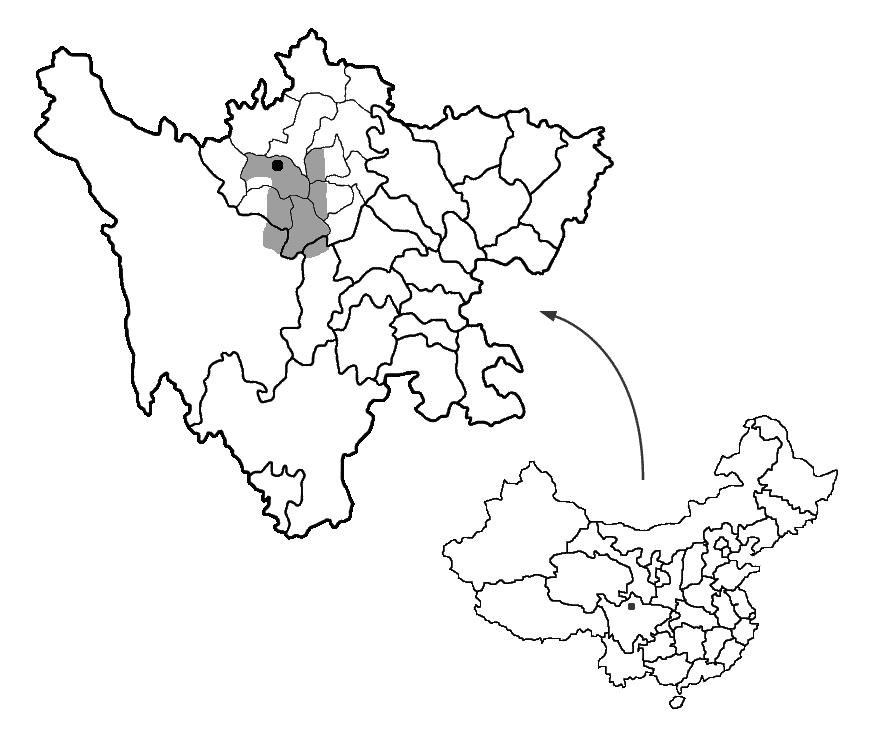
\includegraphics[height=100mm]{carte.JPG}
\caption{Rgyalrong languages}
\label{fig:rgyalrong}
\end{figure}
 

Rgyalrong languages are closely related to Lavrung and Horpa, other neighboring languages, with which they form the \textit{Rgyalrongic} subgroup as demonstrated by \citet{jackson00sidaba}. Rgyalrongic itself is generally considered to belong to a ``Qiangic'' branch including other languages of Western Sichuan such as Pumi, Muya, Queyu, Qiang, Zhaba, Guiqiong, Ersu/Lizu, Shixing and the extinct language Tangut. However, more recent work such as \citealt{jacques.michaud11naish} and \citealt{chirkova12qiangic}, suggests that the Qiangic group as defined is paraphyletic, as the only commonalities between these languages are either symplesiomorphies (common archaisms) or areal features spread through contact. At least Ersu/Lizu and Shixing should be excluded from the Qiangic group, and the status of the other languages is still unclear.
 


Unlike most languages of the Sino-Tibetan family, Rgyalrong languages exhibit a complex head-marking morphology. They have SOV basic word order, and present both accusative and ergative syntactic pivots in different parts of their syntax. The verb distinguishes between singular, dual and plural, but not inclusive/exclusive. Transitivity is unambiguously marked by several affixes and vowel alternations. 

 Tense-Aspect-Modality is marked by a combination of several series of directional prefixes with vowel alternation on the verb root. The structure of the verbal word is illustrated in Table \ref{tab:template:derivational}.
 
   \begin{landscape}
\begin{table}[h]
\caption{The Japhug verbal template (shaded areas indicate derivational prefixes)}\label{tab:template:derivational}
\begin{tabular}{llllll|llllllll|lllll} \toprule
 
\ipab{a-}  &  	\ipab{mɯ- }   &  	\ipab{ɕɯ-}   &\ipab{tɤ-} &  	\ipab{tɯ-}  &  	\ipab{wɣ-}   &

  	 \grise{\ipab{ʑɣɤ-}}  &  	\grise{\ipab{sɯ-}}  & \grise{\ipab{rɤ-}}& \grise{\ipab{nɤ-}} &   	 \grise{\ipab{a-}}   &  	\grise{\ipab{nɯ-}}  &  	\grise{\ipab{ɣɤ-}}  &  	\grise{\ipab{noun}}    &  	 \begin{math}\Sigma\end{math}    &  	\ipab{-t}  &  	\ipab{-a}  &  	\ipab{-nɯ}   &  \\
   &  	\ipab{mɤ-}   &  	\ipab{ɣɯ-}   &\ipab{pɯ-}&  	  &  	 
    & \grise{ }	  &  	 \grise{ }	  &  	  \grise{ }	  &  	   \grise{ }	&  	\grise{\ipab{sɤ-}}&  \grise{ }	 &  	\grise{\ipab{rɯ-}}  &  	 \grise{ }	  &  	  &  	  &  	  &  	\ipab{-ndʑi} &  \\
  &  	   &     &  etc.	  & & 	  &  	  &  	 & &  	  &  	 & &  etc.	  &  	  &  	  &  	  &  	  &  	  &  \\
1  &  	2  &  	3  &  	4  &  	5  &  	6  &  	7  &  	8  &  	9  &  	10  &  	11  &  	12  &  	13  &  	14  &  	15  & 16 &17&18\\
\bottomrule
\end{tabular}
\end{table}
\begin{multicols}{2}
\begin{enumerate}


\item Irrealis  \ipa{a}-- and \ipa{ɯβrɤ}--, Interrogative \ipa{ɯ́}--, conative \ipa{jɯ}--
\item negation \ipa{ma}-- / \ipa{mɤ}-- / \ipa{mɯ}-- / \ipa{mɯ́j}--
\item \textbf{Associated motion \ipa{ɕɯ}-- and \ipa{ɣɯ}--}
\item Directional prefixes ( \ipa{tɤ}--  \ipa{pɯ}--  \ipa{lɤ}--   \ipa{tʰɯ}--  \ipa{kɤ}--   \ipa{nɯ}--   \ipa{jɤ}-- ,  \ipa{tu}--   \ipa{pjɯ}--   \ipa{lu}--   \ipa{cʰɯ}--   \ipa{ku}--   \ipa{ɲɯ}--   \ipa{ju}-- ) permansive  \ipa{nɯ}-, apprehensive \ipa{ɕɯ}-
\item Second person (\ipa{tɯ}--, \ipa{kɯ}-- 2>1 and ta- 1>2)
\item Inverse -\ipa{wɣ}- / Generic S/O prefix \ipa{kɯ}-, Autobenefactive \ipa{nɯ--}, Progressive \ipa{asɯ}-. The inverse and the autobenefactive can be infixed within the progressive \ipa{asɯ}-.
\item Reflexive \ipa{ʑɣɤ}-- 
\item Causative \ipa{sɯ}--, Abilitative \ipa{sɯ}--
\item  Antipassive  \ipa{sɤ}-- / \ipa{rɤ}--
\item  Tropative \ipa{nɤ}--, applicative \ipa{nɯ}--
\item Passive or Intransitive thematic marker \ipa{a}-- / Deexperiencer \ipa{sɤ}--
\item Autobenefactive-spontaneous (appears in this position only when the passive/intransitive determiner is present, otherwise appears in positions 6 and can be infixed in the progressive \ipa{asɯ}--) \ipa{nɯ}--
\item Other derivation prefixes \ipa{nɯ}-- \ipa{ɣɯ}-- \ipa{rɯ}-- \ipa{nɤ}-- \ipa{ɣɤ}-- \ipa{rɤ}--
\item Noun root
\item Verb root 
\item Past 1sg/2sg transitive -\ipa{t} (aorist and evidential)
\item 1sg --\ipa{a}
\item Personal agreement suffixes (--\ipa{tɕi}, --\ipa{ji}, --\ipa{nɯ}, --\ipa{ndʑi})
\end{enumerate}


\end{multicols}
  \end{landscape}


The genesis of this prefixal morphology is poorly known. Some of these prefixes such as the causative \ipa{sɯ}-- and the passive \ipa{a}-- (< *--ŋa--) have clear cognates in other Sino-Tibetan languages and at least part of this template could be very old. However, at least four positions in the template are relatively recently innovated: the negation prefixes (position \textbf{2}), the associated motion prefixes (position \textbf{3}, cf. sections \ref{subsec:associated} and \ref{subsec:grammat}),   the directional prefixes (position \textbf{4}, originate from corresponding locative nouns and adverbs) and  the reflexive \ipa{ʑɣɤ--} (position \textbf{7}, argued by \citet{jacques10refl} to originate from a third person pronoun). 
 
 All inflectional prefixes occur further from the stem than the reflexive, but this is not proof that they are more recently grammaticalized: at least some of them have undergone externalization of inflection (\citealt{haspelmath93extern}). 

The question of word order in Sino-Tibetan languages is also quite controversial. Many researchers, following \citet{li74svo}, have suggested that SOV word order must be reconstructed for proto-Sino-Tibetan, and that SVO languages such as Chinese in the family used to have SOV order, but more recent work such as \citet{dpw07} has shown that this hypothesis is poorly substantiated. 

However, these unsettled historical issues lie beyond the scope of this article, and have no bearing  on the grammaticalization scenario laid out in section \ref{subsec:grammat}, as our discussion focuses only on Rgyalrong languages,  all of which share this prefixal template and a strict SOV typology. Whatever the original word order of proto-Sino-Tibetan, it is clear that Rgyalrong languages have been SOV for a very long time. We find many synchronically opaque noun-verb nominal compounds (as described in \citealt{jacques12incorp}), but not a single example of a verb-noun nominal compound, as would be expected if word order had recently changed. Moreover, there is not a single construction in these languages where verbs are not clause-final.

Very few SOV languages in the world present such a large prefixing template with thirteen prefixing slots; only Athabaskan and Ket seem to share this typological feature. \citet[154-5]{werner97ketisch} posits 14 prefixing slots for Ket, and Athabaskan languages invariably have more than 9 prefixal positions (\citealt[402-405]{rice2000scope}). 



The Japhug verbal structure includes both templatic and layered features, depending on the affixes considered.


We can describe five main templatic features in the Japhug verb, following \citet[10-14]{rice2000scope} and \citet[218]{bickel07inflectional}: discontinuous roots, prohibition against affix recursion, dependency and exclusion between non-adjacent prefixes, metathesis, incompatibilities between prefixes belonging to the same slot.

First, we find some discontinuous roots in Japhug, in the case of intransitive verbs containing the thematic marker -\ipa{a}-; this thematic marker was historically a prefix, but it cannot be analyzed as such for most verbs. See for instance the following example:
\begin{exe}
\ex 
\gll \ipa{ɯʑo}   	\ipa{tɤ-azgrɯ}   	\ipa{nɤ,}   	\ipa{ɯ-taʁ}   	\ipa{tɕheme}   	\ipa{nɯ}   	\ipa{kɤ-a-nɯ-mdzɯ}   	\ipa{nɤ}   \\
he \textsc{aor}-bend.down \textsc{cnj} 3\textsc{sg}-\textsc{top} girl \textsc{top} \textsc{aor}-\textsc{thematic}-\textsc{autoben}-sit \textsc{cnj} \\
\glt He bent down, and the girl sat on him. (Kubzang 76)
\end{exe}
The root of the verb ``to sit'' is \ipa{a-mdzɯ}, but the first element -\ipa{a}- is not the passive, as no corresponding verb without it exists; synchronically, it is a semantically bleached element that must be analyzed as a part of the verb stem. The autobenefactive-spontaneous prefix is therefore actually \textit{infixed} within the verb stem. Lai Yunfan (p.c.) noticed another case of infixation of the autobenefactive-spontaneous prefix in the related Lavrung language.

 
Second, affix recursion is impossible: none of the prefixes in table \ref{tab:template:derivational} can appear more than one time in the verb. 
 

 Third, some affixes depend on the presence of other non-contiguous affixes to occur. For instance, the past transitive 1/2\textsc{sg}>3 --\ipa{t} suffix can only appear if the directional prefix slot is properly filled, and if the verb has the right stem. 
 
 Fourth, some prefixes, such as the autobenefactive-spontaneous \ipa{nɯ}--, undergo metathesis on purely morphological grounds:  \ipa{nɯ}-- occurs in slot 12 if slot 11 is filled; otherwise it appears between slots 6 and 7.  

Fifth, prefixes belonging to the same slot (for instance, directional prefixes and apprehensive) exclude each other. The only exception to this is the inverse prefix, which can be \textit{infixed} within the progressive as in:
\begin{exe}
\ex 
\gll  \ipa{ɲɯ-tɯ-ɤ́<wɣ>sɯ-zgroʁ}    \\
\const{}-2-\textsc{prog}<\inv{}>-attach \\
\glt He is attaching you. (elicitation, Chen Zhen)
\end{exe}


 However, discontinuous dependencies, which are plentiful in the domain of inflectional morphology, are less common in derivational morphology and some phenomena show that some of the prefixes are subject to a layered ordering principle. This is the case in particular of the reciprocal derivation, which can occur both before and after the causative:
 
    \begin{exe}
\ex
\gll   \ipa{sɯ-ɤ-sɯ}$\sim$\ipa{sat} \\
		\caus{}-\recip{}-$\sim$kill \\
\glt to  cause to kill each other.
\end{exe} 
\begin{exe}
\ex
\gll   \ipa{a-sɯ-ɴqʰɯ}$\sim$\ipa{ɴqʰi} \\
		\recip{}-\caus{}-$\sim$dirty \\
 \glt to  cause each other to become dirty.
\end{exe} 


The Japhug template is mostly compatible with \citet{bybee85morpho}'s Relevance Hierarchy:
 
\begin{exe}
\ex  \label{bybee}
person < mood  < tense < aspect < voice < verb stem

\end{exe}
Only two discrepancies with this principle occur in Japhug.

First, in the prefixal chain, the person marker (second person prefix) occurs \textit{closer to the stem} than the irrealis prefix (mood marker) and directional prefixes (mood, aspect and tense markers). 

Second, in the suffixal chain, the 1\textsc{sg} occurs closer to the stem than the past tense marker.


It is interesting to note that in the Athabaskan verb, we find the same discrepancies: the person markers (for subject) are closer to the verb stem than TAM prefixes. However, an interesting difference is the fact that the inverse marker, which can also be used to mark generic agent in Japhug, is closer to the stem than the second person prefix. This goes against the general principle found in Athabaskan (\citealt[245]{rice2000scope}):

\begin{exe}
\ex 
\glt specific reference > non-specific reference 

\end{exe}



\subsection{Associated motion} \label{subsec:associated}
Japhug has a system of ``associated motion'', which includes two prefixes: the translocative \ipa{ɕ-} and cislocative \ipa{ɣɯ-} prefixes, located in slot 3 of the template.

Associated motion is a category first described in various languages of Australia (see \citealt{koch84associated.motion}, \citealt{wilkins91associated.motion}) and more recently applied to the Tacanan languages of South America (see \citealt{guillaume08cavinena}, \citealt{guillaume.associated.motion}). It is also found in other language families, for instance in Algonquian, though with a different terminology (cf. \citealt[729-733]{valentine01grammar} who uses the term ``directional preverb").

This   category refers to grammatical markers that attach to verbs and ``specify that the event denoted by the verb stem is associated with a motion event" as \citet[207]{wilkins91associated.motion} puts it. In some languages, the associated motion system can include up to 14 distinct affixes, distinguished by three main parameters: 1) the deixis (whether the motion is towards the speaker, away from the speaker or unspecified) 2) the syntactic role of the entity undergoing the motion (S/A vs. O) 3) the time of the motion relative to the action expressed by the verb stem (prior, concurrent, subsequent). 

In Japhug, we do not find a system as rich as that described for Arandic or Tacanan languages: only the two prefixes mentioned above are found. Both prefixes are restricted to S/A arguments and to a motion occurring \textit{prior} to the action.


These prefixes are the most common way to express the meanings ``go to'' and ``come to'' in Japhug:
\begin{exe}
\ex 
\gll \ipa{mphrɯmɯ}  	\ipa{ɕ-pɯ-sɯ-re}   	\ipa{tɕe,}   	\ipa{ɕ-tɤ-the}   	\ipa{ra}    \\
 divination \textsc{transloc}-\textsc{imp}-\textsc{caus}-look[III] \textsc{cnj} \textsc{transloc}-\textsc{imp}-ask[III] \textsc{n.pst}:have.to \\
 \glt You have to go to make him do a divination, go to ask him.
 
 \ex
\gll 	\ipa{ɯ-ɕki}   	\ipa{zɯ}   	\ipa{ɣɯ-tɤ-nɯ-thu-nɯ}   	\\
3\textsc{sg}-\textsc{dat}  \textsc{loc}  \textsc{cisloc}-\textsc{imp}-\textsc{autoben}-ask-\textsc{pl} \\
\glt 	Please come  to ask her. (the prince, 66)
\end{exe}



They exhibit S/A accusative alignment: in transitive verbs, the A is always the person doing the motion (coming or going), never the O, even in inverse forms with two human arguments:


\begin{exe}
\ex \label{ex:inverse}
\gll \ipa{nɯ-wa}   	\ipa{nɯ}   	\ipa{to-ɣi}   	\ipa{tɕe,}   	\ipa{ɣɯ-pjɤ́-wɣ-sɯ-ɣe-nɯ}    \\
3\textsc{pl}-father \textsc{top} \textsc{evd:up}-come \textsc{cnj} \textsc{cisloc}-\textsc{evd:down}-\textsc{inv}-\textsc{caus}-come-\textsc{pl} \\
\glt 	Their father came (up) and invited them down (to the Naga realm) (Not: they came to be invited down)
\end{exe}

Unlike corresponding constructions in Tacanan languages, in Japhug associated motion prefix can occur with motion verbs:

\begin{exe}
\ex \label{ex:inverse2}
\gll
\ipa{ɯ-mtɕhi}   	\ipa{ɯ-taʁ}   	\ipa{nɯ}   	\ipa{tɕu}   	\ipa{cɯβjiz}   	\ipa{chɤ-ta,}   	\ipa{tɕe}   	\ipa{ɯʑo}   	\ipa{li}   	\ipa{ɕ-to-ŋke}   	\ipa{tɕe,}    \\
3\sg{}.\poss{}-mouth 3\sg{}.\poss{}-on \topic{} \textsc{loc} flat.stone \textsc{evd:downstream}-put \textsc{coord}  he again \textsc{transloc}-\textsc{evd:up}-walk \textsc{coord} \\
\glt  He put a flat stone on his (brother's) mouth, and went again (to look for water). (Nyima Wodzer, 24)
\end{exe}

These two prefixes are obviously grammaticalized from \ipa{ɕe} ``go" and \ipa{ɣi} ``come''. However, in a strict OV language, grammaticalization into suffixes rather than prefixes would be expected, as is found in complex predicates of other strict OV languages with complex morphology such as Kiranti. For instance in Khaling the verb |kʰoŋ| ``come up" is grammaticalized as a suffix:

\begin{exe}
\ex \label{ex:khaling}
\gll \ipa{dʌrʌm-po} \ipa{kʌ̄m-bi} \ipa{lēːs-kʰɵŋ-ʌtʌ}      \\
 friend-\gen{} house-\loc{} visit.for.a.short.while-come.up-1\sg{}.\pst{} \\
\glt   I came up to visit my friend's house for a short while.
\end{exe}


The translocative \ipa{ɕɯ}-- has four allomorphs \ipa{ɕɯ}--, \ipa{ɕ}--, \ipa{ʑ}-- and \ipa{z}-- conditioned by the nature of the subsequent morpheme in the prefixal chain. The cislocative \ipa{ɣɯ}-- has no allomorphs.

\subsubsection{The motion verb construction}
The grammaticalization of these motion verbs as prefixes rather than suffixes in this SOV language  is all the more surprising if we consider the existence of an alternative  construction in Japhug, a complementation strategy (in  \citet{dixon06complementation}'s sense) with the motion verb occurring \textit{after} the dependent clause:\footnote{A similar construction is described in \citet[488]{sun12complementation}.}
\begin{exe}
\ex \label{ex:supine1}
\gll \ipa{ɯ-fso}   	\ipa{tɕe}   	\ipa{ɬamu}   	\ipa{línɤ}   	\ipa{[pɯwɯ}   	\ipa{ɯ-kɯ-no]}   	\ipa{pjɤ-ɕe,}    \\
 3\textsc{sg}-tomorrow \textsc{coord} Lhamo  again donkey 3\textsc{sg}-\textsc{nmlz:A}-chase \textsc{evd:down}-go \\
\glt The next day, Lhamo went down again to chase the donkey.  (The Raven 62)
\end{exe}

\begin{exe}
\ex \label{ex:supine2}
\gll \ipa{aʑo}   	\ipa{[ndʑi-kɯ-qur]}   	\ipa{chɯ-ɣi-a}   	\ipa{je}   	\ipa{mɤ-phan-a}   	\ipa{nɤ}   	\ipa{mɤ-ʁdɯɣ-a}   	\ipa{thaŋ}    \\
I 2\textsc{du}-\textsc{nmlz:A}-help \textsc{ipf:downstream}-come-1\textsc{sg} \textsc{hort} \textsc{neg}-\textsc{n.pst:}efficient-1\textsc{sg} \textsc{if} \textsc{neg}-harm-1\textsc{sg} \textsc{hypoth} \\
\glt I am coming to help you^d^u, even if I am useless it won't do any harm. (The demon, 19)
\end{exe}

The dependent verb is always in a special non-finite form comprising one or two prefixes depending on the transitivity of the verb. In intransitive verbs, we only find the  nominalization prefix \ipa{kɯ--}, while in transitive verbs we find a combination of this prefix \ipa{kɯ--} with another possessive prefix coreferent with the O. The order is rigid, and the purposive clause cannot be separated from the motion verb.

This is exactly the same form as the S/A nominalization, and this non-finite form occurs in constructions with a few intransitive verbs aside from motion verbs, such as \ipa{ʑɣɤpa} ``to pretend'':
 
  \begin{exe}
\ex
\gll  \ipa{ɯʑo} 	\ipa{kɯ-ngo} 	\ipa{to-ʑɣɤpa,} \\
     she \nmlz{}:S/A-sick \textsc{evd}-pretend \\
  \glt She pretended to be sick. (Nyimawodzer1, 15)
   \end{exe}


 The associated motion forms corresponding to the clauses \ipa{ɬamu	línɤ	pɯwɯ	ɯ-kɯ-no	pjɤ-ɕe} ``Lhamo went down again to chase the donkey'' (\ref{ex:supine1}) and \ipa{ndʑi-kɯ-qur chɯ-ɣi-a} ``I am coming to help you two'' (\ref{ex:supine2}) would be:

  \begin{exe}
\ex
\gll  \ipa{pɯwɯ} \ipa{ɕ-pjɤ-no} \\
      donkey \textsc{transloc}-\textsc{evd:down}-chase \\
   \end{exe}
  \begin{exe}
\ex
\gll  \ipa{ɣɯ-tu-ta-qur-ndʑi} \\
     \textsc{cisloc}-\textsc{ipf}-1>2-help-\textsc{du} \\
   \end{exe}
   
This associated motion construction differs from the motion verb one in three ways.


First, there is a clear difference of semantic scope between the two constructions: the TAM markers in the associated motion construction (example \ref{ex:constr1}) refer to the motion and the action described by the verb root, while in the motion verb construction (\ref{ex:constr2}) they refer to the motion only.

  
   \begin{exe}
\ex \label{ex:constr1}
\gll \ipa{aʑo} \ipa{tɤmtʰɯm} \ipa{ɕ-tɤ-χtɯ-t-a}. \\
I meat \textsc{transloc}-\aor{}-buy-\pst{}-1\sg{} \\
\glt I went to buy meat (and bought it).
  \end{exe}
  
 \begin{exe}
\ex \label{ex:constr2}
\gll  \ipa{aʑo} \ipa{tɤmtʰɯm} \ipa{ɯ-kɯ-χtɯ} \ipa{jɤ-ari-a}. \\
I meat 3\sg{}-\nmlz{}:S/A-buy \aor{}-go[II]-1\sg{} \\
\glt  I went to buy meat (I may or may not have bought it).
  \end{exe}

With the motion verb construction, one can negate the verb in the purposive clause:
 \begin{exe}
\ex \label{ex:constr3}
\gll  \ipa{laχtɕʰa} \ipa{ɯ-kɯ-χtɯ} \ipa{jɤ-ari-a}  \ipa{ri} \ipa{tɤ-χtɯ-t-a} \ipa{maka} \ipa{me} \\
thing 3\sg{}-\nmlz{}:S/A-buy \aor{}-go[II]-1\sg{} but \aor{}-buy-\pst{}-1\sg{} at.all \nonps{}:not.have\\
\glt  I went to buy things \textbf{but did not buy anything}.
\ex \label{ex:constr4}
\gll  \ipa{kɯ-nɯ-rŋgɯ}  	\ipa{jɤ-ari-a}  	\ipa{ri}  	\ipa{kɤ-nɯ-rŋgɯ}  	\ipa{mɯ-pɯ-ŋgrɯ}  	\\  
\nmlz{}:S/A-\auto{}-lie.down 	\aor{}-go[II]-1\sg{}	but	\textsc{inf}-\auto{}-lie.down 	\negat{}-\pst{}.\impf{}-succeed \\
\glt  I went to sleep \textbf{but could not sleep}.
  \end{exe}
  
By contrast, no such option is available with the associated motion prefix. The following sentences are non-sensical and  unacceptable to native speakers:
 \begin{exe}
\ex \label{ex:incorrect2}
\gll  *\ipa{laχtɕʰa} \ipa{ɕ-tɤ-χtɯ-t-a}  \ipa{ri} \ipa{tɤ-χtɯ-t-a} \ipa{maka} \ipa{me} \\
thing \textsc{transloc}-\aor{}-buy-\pst{}-1\sg{} but \aor{}-buy-\pst{}-1\sg{} at.all \nonps{}:not.have\\
\glt  (intended meaning: sentence \ref{ex:constr3}) 
\ex \label{ex:incorrect2}
\gll  *\ipa{ɕ-pɯ-nɯ-rŋgɯ-a}  	\ipa{ri}  	\ipa{kɤ-nɯ-rŋgɯ}  	\ipa{mɯ-pɯ-ŋgrɯ}  \\
\textsc{transloc}-\aor{}-sleep-1\sg{} but	\textsc{inf}-\auto{}-lie.down 	\negat{}-\pst{}.\textsc{ipf}-succeed \\
\glt  (intended meaning: sentence \ref{ex:constr4})

  \end{exe}  

Second, since the complement verb in motion verb constructions is in a non-finite form, all TAM and almost all person marking occurs on the main verb \ipa{ɕe} ``go" and \ipa{ɣi} ``come''. Since these are intransitive verbs  only agreement with the A of the dependent verb occurs, as in example \ref{ex:supine2}, where the main verb \ipa{cʰɯ-ɣi-a} bears the 1\textsc{sg} suffix --\ipa{a}, the A of the dependent verb ``to help''. The O of the dependent verb can only be encoded with the possessive prefix on the non-finite form, as in \ipa{ndʑi-kɯ-qur}. Agreement is therefore split between the two verbs, while in the associated motion construction both are expressed within one single verb form. Although some information about the O is preserved in the motion verb construction thanks to the possessive prefix, one syntactic contrast is lost: that between direct and inverse verb forms, in cases where both arguments are third person. For instance, the verb form \ipa{ɣɯ-pjɤ́-wɣ-sɯ-ɣe-nɯ } ``he came to invite them'' in example \ref{ex:inverse} contains the inverse prefix (see \citealt{jacques10inverse} concerning the pragmatic use of the inverse). The equivalent direct form (used when the agent is more topical than the patient) would be:
  \begin{exe}
\ex
\gll  \ipa{ɣɯ-pjɤ-sɯ-ɣe} \\
      \textsc{cisloc}-\textsc{evd:down}-\textsc{caus}-come \\
   \end{exe}
However, both \ipa{ɣɯ-pjɤ́-wɣ-sɯ-ɣe-nɯ } and  \ipa{ɣɯ-pjɤ-sɯ-ɣe} only have one equivalent in the motion verb construction:
  \begin{exe}
\ex
\gll  \ipa{nɯ-kɯ-sɯ-ɣe} \ipa{pjɤ-ɣi} \\
     3\pl{}.\poss{}-\textsc{nmlz:A}-\textsc{caus}-come \textsc{evd:down}-come\\
   \end{exe}
The contrast between direct and indirect is thus neutralized in the motion verb  construction.

 
Third, in the motion verb construction, the TAM prefixes of the motion verbs indicate direction according to table \ref{tab:directional}.\footnote{See \citet{jackson00sidaba}, who first described a similar construction in the neighbouring Tshobdun language.}
\begin{table}
\caption{Directional prefixes in Japhug Rgyalrong} \label{tab:directional}
\resizebox{\columnwidth}{!}{
\begin{tabular}{llllllllll}
\toprule
TAM & up & down & upstream & downstream & east & west & no direction \\
\midrule
aorist, imperative & \ipa{tɤ--}& \ipa{pɯ--}&\ipa{lɤ--}&\ipa{thɯ--}&\ipa{kɤ--}& \ipa{nɯ--}&  \ipa{jɤ--}\\
aorist 3>3 & \ipa{ta--}& \ipa{pa--}&\ipa{la--}&\ipa{tha--}&\ipa{ka--}& \ipa{na--}&  \ipa{ja--}\\
imperfective & \ipa{tu--}& \ipa{pjɯ--}&\ipa{lu--}&\ipa{chɯ--}&\ipa{ku--}& \ipa{ɲɯ--}&  \ipa{ju--}\\
evidential & \ipa{to--}& \ipa{pjɤ--}&\ipa{lo--}&\ipa{chɤ--}&\ipa{ko--}& \ipa{ɲɤ--}& \ipa{jo--}   \\
\bottomrule
\end{tabular}
}
\end{table}

Non-motion verbs are generally only compatible with one or two non-predictable directional prefixes, and do not normally mark direction. In the motion verb construction, both TAM and direction are marked on the motion verb. For instance, in \ipa{ndʑi-kɯ-qur chɯ-ɣi-a} ``I am coming to help you two'', the prefix \ipa{chɯ--} indicates both imperfective and downstream direction. In the associated motion construction however, only the intrinsic directional prefix on the verb appears. In \ipa{ɣɯ-tu-ta-qur-ndʑi} ``I am coming to help you two'' for instance, we find the imperfective prefix \ipa{tu--} ``up'', as the verb \ipa{qur} always selects the series of prefixes \ipa{tɤ--, ta--, tu--, to--}. Using the \ipa{chɯ--} ``downstream'' directional prefix here would not be correct, and the direction distinction is absent. 

An exception occurs in the case of verbs like \ipa{sɯ-ɣe} ``to cause to come, to invite'' which allow all directional prefixes, as they are motion verbs themselves. In example \ref{ex:inverse}, the form \ipa{ɣɯ-pjɤ́-wɣ-sɯ-ɣe-nɯ } ``he came to invite them'' includes the \ipa{pjɤ--} ``down'' direction prefix, which is not lexically determined in this case, but represents the direction of the action.

Apart from verbs like \ipa{sɯ-ɣe} ``to cause to come, to invite'', which only constitute a small minority, the associated motion construction includes less information than the motion verb one, as it lacks indication of the direction of the action.


The differences between the two constructions can be summarized as follows: (X indicate that a particular combination is possible)

\begin{table}[H]
\caption{Comparison of the associated motion and motion verb constructions in Japhug} \label{tab:comparison}
 \resizebox{\columnwidth}{!}{
\begin{tabular}{llllllllll}
\toprule
 
    &  	S/A agreement   &  	O agreement   &  	direct/inverse   &  	direction   \\  
    \midrule
associated motion  &  	X   &  	X   &  	X   &  	 \grise{}	   \\  
motion verb   &  	X (motion verb)   &  	X (dependent verb)   &  \grise{}	   &  	X   \\  
\bottomrule
\end{tabular} }
\end{table}
The associated motion construction is slightly more informative on person marking, while the motion verb  construction includes directional marking which is lost in the associated motion one. Apart from these minor differences, the semantic and pragmatic distinctions between the two constructions are fairly subtle. 

The relative frequency of the two constructions can be informative. In the following table, we indicate the number of occurrences of verb forms with either an associated motion prefix or a motion verb construction in a corpus of 30 texts.\footnote{These texts include mainly traditional stories, some procedural texts and one conversation. It only includes half of our total text corpus.} We classified all occurrences into six categories depending on the transitivity of the verb, the presence of an overt object (for transitive verbs) and the presence of an overt locative phrase corresponding to the direction of the motion indicated by the associated motion prefix or the motion verb.

Ambiguous cases (in particular transitive or intransitive verbs with a dative argument) have been excluded from the table.

\begin{table}[H]
\caption{Frequency of the associated motion   \ipa{ɕɯ}-- / \ipa{ɣɯ}-- prefixes vs. motion verbs constructions with  \ipa{ɕe} /  \ipa{ɣi} in Japhug texts} \label{tab:comparison.texts}
 \resizebox{\columnwidth}{!}{
\begin{tabular}{llllllllll}
\toprule
&overt O,  & overt O,  & covert O,&covert O,  & intransitive, &intransitive, &total\\
&overt locative&covert locative& overt locative &covert locative&overt locative&covert locative \\
\midrule 
  \ipa{ɕɯ}-- & 8	&37	&4	&22	&9	&24 &104 \\
 \ipa{ɣɯ}-- &  1	&5	&2	&7& 0	&1 & 16\\

 \midrule
\ipa{ɕe} &0	&15&	1&	7&1	&17&41\\
 \ipa{ɣi} &0	&7&	1	&7&0&3&18\\
\bottomrule
\end{tabular} }
\end{table}

We have also compared the relative frequency of the two constructions with imperatives on the same corpus of texts:\footnote{However, the verbs with dative arguments have been included.}
\begin{table}[H]
\caption{Frequency of the associated motion vs. motion verb constructions in imperative forms} \label{tab:comparison.texts}
 
\begin{tabular}{llllllllll}
\toprule
&& imperative forms &total of occurrences \\
\midrule
 associated& \ipa{ɕɯ}-- & 47 & 120\\
motion & \ipa{ɣɯ}-- &  12 &34\\

 \midrule
motion verb &\ipa{ɕe} &2&45\\
& \ipa{ɣi} &1&36\\
\bottomrule
\end{tabular}  
\end{table}
These data reveal three facts. First, the motion verb construction is two times less common than the associated motion one. The greater frequency of the associated motion construction is linked with the fact that it is often used in contexts where a motion verb would not be used in a Western language:
  \begin{exe}
\ex \label{ex:tu}
\gll  \ipa{ŋotɕu}   	\ipa{ɕ-pɯ-tɯ-tú-nɯ?}   	\\
where \textsc{transloc}-\textsc{pst.ipf}-3-be.there-\textsc{pl} \\
\glt Where have you been? (The prince, 56)
   \end{exe}
  \begin{exe}
\ex \label{ex:sWru}
\gll  \ipa{rgɯnba}   	\ipa{jɤ-ɕe}   	\ipa{tɕe,}   	\ipa{mphrɯmɯ}   	\ipa{ɕ-pɯ-sɯ-re}   	\ipa{nɤ,}   	\ipa{ɯ-ɲɯ́-phɤn}   	\ipa{kɯ}    \\ 
temple \imp{}-go \textsc{coord} divination \textsc{transloc}-\textsc{imp}-\textsc{caus}-practive.divination \textsc{coord} \textsc{qu}-\textsc{const}-be.effective \textsc{dubitative}\\
\glt Go to the temple and ask (the monk) to make a divination, maybe it will work. (Divination, 40)
   \end{exe}

Second, motion verbs constructions are very rare with imperatives, and associated motion prefixes are more commonly used.
 
Third, clauses including an overt locative phrase corresponding to the direction of the motion more commonly include associated motion constructions: out of 27 examples in the corpus, 24 have a verb with associated motion prefix, and only 3 use a motion verb. 

In conclusion, the motion verb construction is clearly the least grammaticalized  construction of the two, and is mainly used to focus on the motion itself rather than on the subsequent action or on the place towards which the motion is directed.

\subsubsection{Motion verb constructions in related languages}
While the prefixal associated motion construction is restricted to Rgyalrong languages among languages of the ``Qiangic" group, similar motion verb constructions are found in other closely related languages such as Pumi (\ref{ex:pumi}, \citealt{jacques11pumi.tone}) and the extinct language Tangut (\ref{ex:tangut}):
\begin{exe}
\ex  \label{ex:pumi}
\gll \ipa{hmĩ³-ʂə̃¹-mə̃dərə} \\
beg-go-\textsc{nar} \\
\glt He went to beg. (Divination with a pig head, 17)
\end{exe}



\begin{exe} 
\ex    \label{ex:tangut}
\gll  \ipa{nji²nji²} 	\ipa{tɕhjụ¹.ji¹} 	\ipa{zeew²} 	\ipa{tɕhjiw¹thwər¹} 	\ipa{.jij¹} 	\ipa{nji¹} 	\ipa{do²} 	\ipa{tha¹} 	\ipa{sja¹} 	\ipa{ɕjɨ¹} 	\ipa{phji¹}  \\
		 secretly Chu.Ni send Zhao.Dun \gen{} house \textsc{all} oppress kill  go[B] cause[A]\\
\glt  \begin{tabular}{lllllllllll}
\tgf{3627} & 	\tgf{3627} & 	\tgf{1796} & 	\tgf{3119} & 	\tgf{5871} & 	\tgf{5093} & 	\tgf{4633} & 	\tgf{1139} & 	\tgf{2862} & 	\tgf{5447}  &\tgf{1394}\\
  \tgf{4225} & 	\tgf{4481} & 	\tgf{0749} \\
\end{tabular}\\
\glt He secretly sent Chu Ni to kill Zhao Dun. (Leilin, 03.95A.6-7)
\end{exe}



This suggests that the motion verb construction found in Japhug is not a recent innovation, but was present in the proto-language. However, it also raises the question of how Japhug could have developed its   cis- and translocative prefixes, as simple agglutination of the two verbs should have resulted in associated motion \textit{suffixes}, not prefixes.

\subsection{Alternative path of grammaticalization} \label{subsec:grammat}
As seen in the previous subsection, it is unlikely that the associated motion prefixes originate from a structure resembling the motion verb construction. The obvious alternative, following \citet{comrie80morpho}'s insight, is to look for another potential construction where motion verbs appear before, not after the lexical verb. One possibility could be right-extraposition of the dependent verb. Such phenomena are not common in Rgyalrong, but examples can be found in texts:
\begin{exe}
\ex  
\gll\ipa{tɕhi}   	\ipa{tu-tɯ-ste}   	\ipa{ŋu}   	\ipa{kɤ-sɤ-fstɯn}    \\
what \textsc{ipf}-2-do.this.way[III] \textsc{n.pst}:be \textsc{inf}-\textsc{antipass}-serve \\
\glt How do you serve people? (Kunbzang 128)
\end{exe} 
Here the non-finite  verb \ipa{kɤ-sɤ-fstɯn} is extraposited after the main verb and its TAM auxiliary. The normal word order would be:
\begin{exe}
\ex  
\gll \ipa{kɤ-sɤ-fstɯn}   	\ipa{tɕhi}   	\ipa{tu-tɯ-ste}   	\ipa{ŋu}   	 \\
\textsc{inf}-\textsc{antipass}-serve what \textsc{ipf}-2-do.this.way[III] \textsc{n.pst}:be  \\
\end{exe} 
 
 However, in view of the rarity of such constructions, and given the fact that no example involving a motion verb has been found, this does not seem to be the most likely explanation to account for the genesis of the associated motion prefixes.

On the other hand, \citet[141]{givon2000internal} suggested that some of the prefixes in the Athabaskan template originate from verbs, that were incorporated following a \textit{serial verb construction}. 

In the case of Rgyalrong languages, two possibilities can be contemplated: either coordinated clauses or a serial verb construction.\footnote{A third possibility, involving a motion verb in converbal form followed by a fully finite lexical verb, is also possible, but seems unlikely as converbial constructions are relatively uncommon in Rgyalrong languages. }

	The first hypothesis entails the coalescence of two independent clauses fulfilling the following conditions: (a) the first clause includes a motion verb ``to come" or ``to go" and the order of the clauses reflects the temporal order of the action; (b) both clauses share the same S/A; (c) the second clause is reduced to a single verb, without overt agent, patient or complement of any sort.  Such clauses are possible in Japhug:

\begin{exe}
\ex  \label{ex:buy}
\gll   \ipa{kɤntɕhaʁ} \ipa{jo-ɕe} \ipa{tɕe} \ipa{to-rɤ-χtɯ} \\
  street \evd{}-go  \textsc{coord} \evd{}-\textsc{antipassive}-buy\\
\glt He went down the street (to the market) and  bought things. (Elicitation, Chenzhen)
\end{exe}

In Japhug such structures are not common in natural texts. When the motion verbs ``to come" and ``to go" precede  another verb, we commonly find an echo phenomenon, whereby the verb takes the associated motion prefix corresponding to the motion verb  (cf. examples \ref{ex:inverse} and \ref{ex:sWru}).\footnote{I thank Antoine Guillaume for pointing this fact to my attention.} However, sentence \ref{ex:buy} is accepted as correct by native speakers without hesitation, though not with all verbs (in particular it would be difficult to use the basic transitive verb \ipa{to-χtɯ} ``he bought it" in place of the antipassive form). Two verbs cannot following each other in such constructions without an intervening coordinator like \ipa{tɕe}.

Such an attested structure could coalesce into one word following the path proposed in \ref{ex:CkonWrNgW} (using the intransitive verb \ipa{rŋgɯ} ``to sleep" as an example, presented here in  modern Japhug pronunciation rather than in reconstructed proto-Rgyalrong for convenience):

\begin{exe}
\ex   \label{ex:CkonWrNgW}
\begin{xlist}
\exi{(a)} 
\gll *ju-ɕe tɕe ku-nɯ-rŋgɯ >  \\
\textsc{ipf}-go \textsc{coord} \textsc{ipf}-\textsc{autobenefactive}-sleep   \\
\exi{(b)} 
\gll  *ju-ɕe-ku-nɯ-rŋgɯ > \\
 \textsc{ipf}-go-\textsc{ipf}-\textsc{autobenefactive}-sleep    \\
\exi{(c)} 
\gll  *ɕe-ku-nɯ-rŋgɯ > \\
 go-\textsc{ipf}-\textsc{autobenefactive}-sleep   \\
 \exi{(d)} 
\gll   \ipa{ɕ-ku-nɯ-rŋgɯ} \\
  \textsc{transloc}-\textsc{ipf}-\textsc{autobenefactive}-sleep \\
\glt He goes to sleep.
\end{xlist}
\end{exe}
Stage (a) is not really reconstructed, as it still exists (though marginally) in modern Japhug; we have no way to know whether the coordinator \ipa{tɕe} existed in a former stage of the language, and at this stage parataxis may have also been possible. In stage (b), the coordinator is lost and both verbs tend to merge phonologically. While at stage (a) the two verbs were  independent heads, by stage (b) they have fused into a single predicate. In stage (c), the first TAM prefix is lost. 

Alternatively, it is possible to propose that associated motion prefixes originate from a serial verb   constructions.
Such constructions were first described in Rgyalrong by \citet[490]{sun12complementation}, and they especially occur with deideophonic verbs as in the following   example:

\begin{exe}
\ex  
\gll \ipa{pɯ-ɣɤzgrɤɣlɤɣ-nɯ}   	\ipa{pɯ-rɟaʁ-nɯ}    \\
  \aor{}-make.a.rythmic.jumping.noise-\pl{} \aor{}-dance-\pl{}\\
\glt They made much noise as they danced.  (Elicitation, Dpalcan)
\end{exe}
We also find  lexicalized serial constructions such as \ipa{-stu -mbat} ``to try hard'':
\begin{exe}
\ex  
\gll \ipa{tɤ-stu}   	\ipa{tɤ-mbat}    \\
\textsc{imp}-try.hard \textsc{imp}-try.hard \\
\glt  Try hard!
\end{exe}
Both verbs have the same TAM and person markers, and no conjunction can occur between them.

No such serial verbs construction exist for motion verbs. However, a construction of this type could be hypothesized instead of coordination at stage (1) of \ref{ex:CkonWrNgW}.

These two hypotheses (coordinated clauses and serial verb construction) are not mutually exclusive,  as a serial verb construction might have been an intermediate stage between independent clauses and associated motion construction, and differ little at least as far as surface forms are concerned.

The grammaticalization of the associated motion prefixes, regardless of their exact origin, is at least a common Rgyalrong innovation (more work is required to determine whether traces of these prefixes exist in Lavrung and Horpa). Not only traces of cognate prefixes are found in all four Rgyalrong languages (Japhug, Tshobdun, Showu and Situ), but we also find idiosyncrasies. For instance, the transitive verb ``to bring, to fetch'' (Japhug \ipa{ru}, Bragdpar Situ \ipa{ró} / \ipa{rô}) must appear with an associated motion prefix (indicated here in bold) in all Rgyalrong languages:\footnote{This verb may be etymologically related to the homophonous intransitive \ipa{ru} ``to look at'', which can also take associated motion prefixes.}

\begin{exe}
 \ex  
 \gll  \ipa{\textbf{ɕ}-tɤ-ru-t-a}  (Japhug) \\
 \textbf{\textsc{transl}}-\aor{}:\textsc{up}-bring-\pst{}-1\sg{} \\
\ex  
 \gll  \ipa{rə-\textbf{ɕɐ}-rô-ŋ}  (Situ) \\
 \aor{}:\textsc{up}-\textbf{\textsc{transl}}-bring.\textsc{aor}-1\sg{} \\
\glt I fetched it.
\end{exe}
This cognate construction is too specific  to be the result of parallel development, and must be inherited from proto-Rgyalrong. However, Situ differs from all other Rgyalrong languages in that the associated motion prefixes appear between the verb stem and the TAM directional prefixes.

In the Cogtse dialect of Situ Rgyalrong, although    no associated motion prefixes have been described, we find a prospective \ipa{po-} prefix as shown by \citet[268]{youjing03zhuokeji}, homophonous with the verb ``to come''. 
\begin{exe}
\ex  
 \gll \ipa{khrī}   	\ipa{ko-po-smên}    \\
rice \textsc{pfv}-\textsc{prov}-be.cooked[II] \\
\glt [The speaker opens the lid of the cooker and then says] The rice is about to be cooked.
\end{exe}

  Cogtse Situ represents a further stage of grammaticalization, and we have to suppose the following path:
\begin{exe}
\ex  
 \glt verb ``to come'' > cislocative > prospective
\end{exe}
For the semantics, note the change of the venitive into a future in Iraqw according to \citet[308-9]{heine-kuteva02}.

The presence of this prefix in a different templatic position in both Situ dialects \textit{after} the directional/TAM prefixes is all the more interesting because it goes against Bybee's Relevance Hierarchy (\ref{bybee}), since a mode marker gets closer to the verb stem than an aspect marker. It also contradicts both of Hawkins' principles (\ref{ex:hawkins}), as we observe that, given two competing constructions (the motion verb construction and the serial verb construction), the more   marginal serial verb construction was the one that gave rise to the associated motion prefixes.


Unlike the case of the Mongolic languages studied by Comrie, none of the alternative explanations (phonological structure, adjacency or contact) are applicable to account for the Japhug case:

First, there is no phonological constraint against unstressed suffixes or head-dependent structures with unstressed dependent in Japhug (see slots 17 and 18 of the verbal template). In some languages of the Sino-Tibetan and Mon-Khmer families, we do find \textit{sesquisyllables} or iambic syllable structures, where words are either monosyllabic or monosyllabic with a weak unstressed syllable with undetermined vowel; \citet{donegan04munda} argued that the shift from this type to the trochaic type in Munda caused the dramatic change from a prefixing to a suffixing language. 

The presence of unstressed prefixes with schwa-like vowels (/ɯ/ and /ɤ/) in Japhug could lead to the conclusion that Japhug  should also be treated as a language with sesquisyllabic structure. In such a language, grammaticalizing an unstressed morpheme as a suffix would go against the main prosodic structure of the language, and explain why the construction leading to a prefixing form was favored over the other one in the grammaticalization process.

However, as pointed out by \citet{michaud12mono}, Japhug cannot be analyzed as a language with sesquisyllabic structure; rather, it is in a pre-sesquisyllabic stage, where true polysyllables with full vowel and consonant contrasts on several syllables exist, and where prefixes can actually be stressed.\footnote{For instance, the inverse prefix shifts stress onto the preceding prefix.} The hypothesis that preference for prefixes in Japhug would be due to the phonological structure of this language is therefore inconclusive.

Second, no element can be inserted between the motion verb and the dependent verb in the motion verb construction, so that adjacency is never broken, unlike in Mongolic languages where in the SOV construction, the S is often separated from the verb. This argument cannot be applied to Japhug.
 
Third, none of the languages in contact with Rgyalrong (Northern Qiang, Amdo Tibetan and Sichuan Chinese) present associated motion prefixes: this category is therefore unlikely to have developed under areal influence.


 
\section{Conclusion}
In this paper, we sought to examine the question whether Hawkins' Head Ordering Principle and Processing Preference for Suffixes Principle can be shown to play a role in diachronic development.

In the second section, we   show  that potential cases of harmonization of affix order are inconclusive, as either additional factors can be proposed to explain the phenomena in question (phonological constraints, adjacency of words in the proto-language or areal influence) or the purported morphological change is still hypothetical.

In the third section,  we  documented a case of prefix creation in a strict SOV language which apparently contradicts Hawkins' two principles.  In Japhug, coordinated clauses involving a motion verb and a lexical verb were grammaticalized into a single predicate, resulting in a disharmonious (SOV-prefixing)   construction. On the other hand, the subordinating (lexical verb + motion verb) construction did not grammaticalize into a single predicate, though this would have lead to a harmonious construction (SOV-suffixing). Unlike the cases of harmonization, no additional factor can be proposed to explain this unusual grammaticalization.

One single counter-example is enough to disprove an absolute constraint: this work shows that disharmonious grammaticalization is possible even in a language with strict word order, and that Hawkins' Head Ordering Principle as such has no verifiable influence on language change. It is likely that similar cases of disharmonization can be found in Athabaskan, in particular the prefixes thought by \citet[141]{givon2000internal} to originate from the first member of a serial verb construction.

The Rgyalrong data studied in this article also prove that SOV languages can develop prefixing morphology without the need of a VO stage, and that prefixes can thrive in a verb-final environment; in more general terms, this implies that inferring the word order of a proto-language from the affix order of its daughter languages is impossible.


\bibliographystyle{myenbib}
\bibliography{bibliogj}
\end{document}